\chapter[\paperVtitle]{\texorpdfstring{%
		\paperVtitle}{%
		\paperVtitle}}
\label{ch:recsyssgx}
\paperRemark{\paperVref} % TODO: consider adding e.g. Reformatted for clarity

{

% IEEE CS
%\documentclass[conference,compsoc]{IEEEtran}
%\usepackage{cite} % apparently should be used with IEEE CS?

%\usepackage{todonotes}

%\usepackage{amsmath,amssymb,amsfonts}
%\usepackage{booktabs}
%\usepackage{tikz}
%\usetikzlibrary{calc,shapes}

%\begin{document}

%
% The "title" command has an optional parameter, allowing the author to define a "short title" to be used in page headers.
%\title{Privacy-enabled Recommendations for Software Vulnerabilities}

%\author{\IEEEauthorblockN{Linus Karlsson}
%	\IEEEauthorblockA{Dept. of Electrical and Information\\
%		Technology, Lund University\\
%		Lund, Sweden\\
%		linus.karlsson@eit.lth.se}
%	\and
%	\IEEEauthorblockN{Nicolae Paladi}
%	\IEEEauthorblockA{Dept. of Electrical and Information\\
%		Technology, Lund University\\
%		Lund, Sweden\\
%		nicolae.paladi@eit.lth.se \\ RISE Research Institutes of Sweden}}

%\maketitle

\section*{Abstract}
New software vulnerabilities are published daily.
Prioritizing vulnerabilities according to their relevance to the collection of software an organization uses is a costly and slow process.
While recommender systems were earlier proposed to address this issue, they ignore the security of the vulnerability prioritization data.
As a result, a malicious operator or a third party adversary can collect vulnerability prioritization data to identify the security assets in the enterprise deployments of client organizations. 
To address this, we propose a solution that leverages isolated execution to protect the privacy of vulnerability profiles without compromising data integrity.
To  validate an implementation of the proposed solution we integrated it with an existing recommender system for software vulnerabilities.
The evaluation of our implementation shows that the proposed solution can effectively complement existing recommender systems for software vulnerabilities. 

\section{Introduction}
\label{sec:introduction}

Modern enterprise software systems are increasingly complex.
Organizations commonly use a plethora of software systems - running either in-house or in public clouds - running on hundreds or thousands of devices.
A simple and carefully implemented software library may run in isolation for extended periods of time without maintenance.
However, as more and more software applications are interconnected, they must be adapted to support new communication protocols, updated to process new types of input data, and patched to fix vulnerabilities.
Software patching is costly, since it requires specialist human effort and must be done shortly after vulnerabilities are discovered - often during weekends and evenings - in order to minimize the risk of exploits.
Since software vulnerabilities can be discovered on any layer of the software stack, the cost is compounded by the complexity of selecting and prioritizing the patches.

Information about software vulnerabilities is collected from several sources, such as public or private security information providers, security researchers or software vendors.
Vulnerabilities discovered by the vendor of the respective software are often treated as software bugs and corrected in the regular release cycle.
Other vulnerabilities, discovered by software users or security researchers, are either communicated directly to the vendors, publicly released, or sold as zero-day exploits.
Publicly known vulnerabilities are assigned a common vulnerability and exposure (CVE) identifier, along with high-level attributes such as: 
perceived impact on confidentiality, integrity, and availability; 
attack complexity; 
attack vector; 
and required privileges.
With new vulnerabilities published daily, software users must review the relevant vulnerabilities, understand their impact and prioritize them. 
This makes prioritizing software vulnerabilities a stringent issue for both software vendors and software users.

Recommender systems \cite{aggarwal:2016} were earlier proposed as solutions for vulnerability prioritization~\cite{bozorgi:2009,farris:2018,cobleigh:2018}.
However, \textit{vulnerability profiles}, i.e. the priority ranking of vulnerability entries, reveal valuable information about the software libraries, packages, applications and protocols that are part of the user's \textit{software bundle}, i.e. the collection of software applications, services and protocols an organization uses.
Access to this information allows an adversary to build an intimate profile of an organization's internal systems - including specific software packages, versions and configurations.
This enables highly effective, targeted attacks using zero-day exploits.
While the recommender systems proposed earlier address to some extent vulnerability prioritization, they do not implement mechanisms to protect the vulnerability profiles.
We address this by describing the design, implementation and evaluation of a privacy-preserving mechanism for software vulnerability recommender systems.
We leverage commodity isolated execution environments to protect vulnerability profiles using an approach derived from earlier work on differential privacy~\cite{dwork:2006}, yet without compromising the integrity of vulnerability data.
%\subsection{Contribution}
%\label{subsec:contribution}
Our contribution is as follows:
\begin{itemize}
    \item We describe a privacy protection mechanism to protect client vulnerability profiles;
    to the best of our knowledge, this is the first work addressing the privacy of client vulnerability profiles.
    \item we describe the implementation and evaluation of a prototype solution, implemented using Intel SGX enclaves and tested with a functioning vulnerability recommender system.
\end{itemize}

%\subsection{Paper Organization}
%\label{subsec:paper-organization}
The remainder of this paper is organized as follows.
We introduce the background, including the system model and the threat model in section~\ref{sec:vulnerability-management}.
We discuss the solution space for protecting vulnerability profile privacy in Section~\ref{sec:solution},
describe the implementation in Section~\ref{sec:recsyssgx:implementation} and present the evaluation results in Section~\ref{sec:recsyssgx:evaluation}.
Finally, we discuss the related work in Section~\ref{sec:related} and conclude in Section~\ref{sec:recsyssgx:conclusion}.

\section{Preliminaries}
\label{sec:vulnerability-management}
We follow earlier work and define \textit{software vulnerabilities} as exploitable software flaws in software systems that pose security risks~\cite{bozorgi:2009, frei:2010}.
Frei et al. describe several distinct phases of the vulnerability life-cycle: creation, discovery, exploit availability, public disclosure, patch availability, and patch installation.
The life-cycle events are grouped into three risk exposure phases: pre-disclosure, post-disclosure, and post-patch~\cite{frei:2010}.
In the pre-disclosure phase, neither vendors nor users can affect the impact of an externally discovered security vulnerability.
Once a vulnerability is disclosed (either by the vendor itself or externally), vendors and users can develop patches to correct the vulnerability, or alternatively mitigate it through workarounds.
In the scope of this paper, we consider software vendors as the only legitimate source of software patches.
Considering the large number of software vulnerabilities released on a daily basis, assessing the impact of a vulnerability on a particular software bundle is a tedious task.
While the community proposed a variety of approaches for vulnerability risk assessment~\cite{sridharan:2008} they are often ad-hoc, do not scale, and are not sufficiently robust to reflect the complexity of enterprise environments.

\textit{Automating} vulnerability prioritization can reduce the duration and the risk exposure of the post-disclosure phase.
Rapid prioritization of software vulnerabilities can both speed up patch development and patch installation.
However, despite increasing productivity, software vulnerability recommenders pose data privacy risks as they may leak client vulnerability  profiles, including information about software vulnerabilities that users and vendors consider of primary interest.
We address this by proposing an approach to protect client vulnerability profiles in software vulnerability recommenders. 
We next describe the system model of automated vulnerability prioritization followed by the treat model we consider in this work.

\subsection{Automating Vulnerability Prioritization}
\label{subsec:scenario}
Automatic tools to provide software vulnerability recommendations have been described earlier~\cite{farris:2018,cobleigh:2018}.
Such tools help enterprise customers with recommendations and are often provided in a Software-as-a-Service (SaaS) delivery model.
A key component in this scenario is that the service provider must have knowledge both about the customers' software bundles and of customer data such as user preferences from historic interactions with the system.

We consider the scenario described below.
The service provider offers two distinct features: \textit{vulnerability identification}, and \textit{vulnerability prioritization}.
The output of vulnerability identification is a list of vulnerabilities, encoded as CVE identifiers.
In the following step, the vulnerability prioritization step, the list of CVE identifiers is passed to a recommender, which then ranks the list of CVEs according to user preferences.
Output from the identification phase can be obtained from various sources \cite{githubsecalert,farris:2018,cobleigh:2018}.
In this paper we focus on the vulnerability prioritization phase.

Clients require a profile shared with a service provider in order to enable the recommender system to provide personalized ranking in the prioritization phase.
This profile contains the client's individual preferences, including client considerations while assessing the severity of a vulnerability.
We consider the scenario illustrated in Figure~\ref{fig:vuln-prio-scenario}.
A client requests recommendations for a given set of CVE identifiers from the recommender system.
To get personalized recommendations, the client also attaches its client profile $p$ to the request.
The recommender returns a personalized ranking $r$ of the given vulnerabilities.
Note that in this scenario, the recommender can trivially map a client to its profile;
there is no data privacy.

\begin{figure}[ht]
	\centering
	\begin{tikzpicture}[scale=1, every node/.style={scale=1}, node distance=1cm, font=\footnotesize\sffamily]
		\node[draw,minimum height=1cm] (client) at (0,0) {Client};
		\node[draw,minimum height=1cm,right=of client] (recommender) {Recommender};
		
		\draw[->] ([yshift=0.3cm]client.east) -- node[above] {$p$, cves} ([yshift=0.3cm]recommender.west);
		\draw[<-] ([yshift=-0.3cm]client.east) -- node[below] {$r$} ([yshift=-0.3cm]recommender.west);
	\end{tikzpicture}
	\caption{Vulnerability prioritization: a client requests recommendations for a set of CVEs, using client profile $p$}
	\label{fig:vuln-prio-scenario}
\end{figure}

\subsection{Isolated Execution}
\label{subsec:isolatedexecution}
In this paper we propose a mechanism to protect the privacy of client requests to the recommender.
This mechanism requires confidentiality of the data, requirements that can be satisfied using isolated execution. 
We use SGX enclaves~\cite{anati:2013,mckeen:2013,xing:2016,mckeen:2016} to create commodity trusted execution environments (TEEs) during operating system run-time.
We use TEEs to protect the privacy of client vulnerability profiles.
SGX enclaves rely on a trusted computing base of code and data loaded at enclave creation time, processor firmware, and processor hardware.
Program execution within an enclave is opaque to the underlying operating system and other mutually distrusting enclaves on the platform.
Enclaves operate in a dedicated memory area called the Enclave Page Cache, a range of dynamic random access memory that cannot be accessed by system software or peripherals~\cite{mckeen:2013}.
The CPU firmware and hardware are the root of trust of an enclave.
Isolation features implemented in firmware and hardware prevent access to the enclave's memory by the operating system and other enclaves.
While we use Intel SGX enclaves in our implementation of the privacy-preserving service, alternative commodity TEEs~\cite{mofrad:2017, brasser:2019} may be used.

\subsection{Threat Model}
\label{subsec:threat-model}

To construct a correct and relevant threat model in the scenario described above, we conducted in-depth interviews with software vendors and users that operate enterprise deployments.
Software vendors highlight the importance of protecting information about relevant software vulnerabilities during the pre- and post-disclosure phases, i.e. while assessing the vulnerability impact and prioritizing it, as well as before releasing a software patch (see Figure~\ref{fig:conf-window}).
We aim to protect the confidentiality of the vendor's software vulnerability priority ranking, since it reveals information about the severity of the vulnerability (as perceived by the vendor) and can be used to guide exploit development.
We assume clients have no information about unpublished vulnerabilities.
Hence, we must protect the confidentiality of the relevance and priority of the released security patches during the post-disclosure (denoted as $t_{pd}$) and post-patch (denoted as $t_{pp}$) phases, i.e. up to the point when software users patch their systems.
%===========================================================================
\begin{figure}[h]
  \centering
  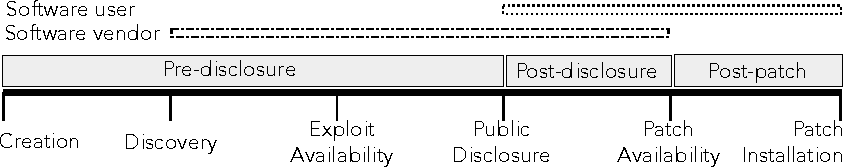
\includegraphics[width=\linewidth]{confidentiality-window}
  \caption{Vulnerability confidentiality window}
  \label{fig:conf-window}
\end{figure}
%===========================================================================

We assume the duration of the post-disclosure and post-patch phases is constant, equal to $T$:
\begin{equation}
    t_{pd} + t_{pp} = T
\end{equation}

The proposed architecture contains three main components - Client, Intermediary and Recommender.
We describe the security assumptions about the components of the proposed architecture.
\subsubsection*{Client}
The Client is potentially malicious, and may submit queries containing requests for arbitrary CVE identifiers.
The goal of the malicious Client is to reveal the privacy-preserving algorithm implemented in the Intermediary and distinguish the vulnerability profiles of other Clients from the vulnerability profiles generated by the Intermediary.
A set of Clients may collude to achieve this purpose.

\subsubsection*{Recommender}
The Recommender is an \textit{honest-but-curious} entity that aims to reveal the vulnerability profile of a specific Client.
The Recommender is assumed to have access to powerful computation capacity and is not sensitive to changes in the computation load of the queries received from the Client.
A collusion between the Client and the Recommender reveals the vulnerability profile of the colluding Client and is out of the scope of this model.

\subsubsection*{Intermediary}
The Intermediary is potentially malicious and aims to reveal the vulnerability profile of a specific Client.
A collusion between the Client and the Intermediary reveals the vulnerability profile of the colluding Client and is out of the scope of this model.
However, we consider that the isolated execution enclave that hosts the privacy protection mechanism is trustworthy;
its trustworthiness can be established through remote attestation by any of the components participating in the protocol.
Isolated execution enclaves used in the implementation of the Intermediary are vulnerable to side-channel attacks~\cite{wang:2017};
we explicitly exclude side-channel attacks from this threat model, since they can be mitigated through improved software implementation.

We consider a remote adversary with attack capabilities on the network and platform level.
The adversary is capable to observe and interact with the network communication between Client and the Recommender, as well with the communication among the internal services of the Recommender.
Furthermore, the adversary can launch arbitrary processes and obtain root access on the hosts running the Recommender.

\section{Vulnerability Profile Privacy}
\label{sec:solution}

As discussed in Section~\ref{subsec:threat-model} above, our goal is to protect the privacy of individual Client vulnerability profiles.
To design a solution for this task, we consider the following defining aspects: 
\textit{(i)} Client profile updates are sparse (e.g. one request every period $T$); 
\textit{(ii)} vulnerability profiles evolve after every period $T$;
\textit{(iii)} the value of an arbitrary snapshot of the vulnerability profile decays in time $T$, equal to the length of software user's confidentiality window.
These are aspects that are sound in the context of vulnerability prioritization, but may not hold for other recommender systems.

While a myriad of definitions, approaches and techniques have been proposed for privacy protection, it remains an elusive goal.
One reason is the discrepancy between the assumptions required for a solution to offer data privacy protection in the presence of other related data sets.
Another reason is the trade-off between data privacy and data utility present in most privacy-preserving solutions~\cite{dwork:2006, dwork:2014}.

To protect the privacy of Client vulnerability profiles, we design an approach based on a combination of k-anonymity~\cite{samarati:1998, samarati:2001} and local differential privacy~\cite{bassily:2017, tang:2017, zheng:2017}.
A combination of the two approaches guarantees that queries derived from Client vulnerability profiles are released only in large enough batches that contain additional queries derived from statistically different pseudo vulnerability profiles.
This approach prevents the direct release of information about subgroups and provides differential privacy guarantees by adding pseudo-random noise (in the form of fake queries) to the genuine queries based on individual Client vulnerability profiles.

This approach, adapted to the vulnerability recommender system described in~\cite{cobleigh:2018}, allows us to substitute the privacy-utility trade-off with a privacy-cost relation.
Intuitively, larger proportions of noise accompanying genuine queries lead to stronger privacy of the respective Client vulnerability profile.
While increasing computational cost of the recommender, this allows to proportionally decrease the utility of information observed by the adversary, without utility loss for the client.

\subsection{k-anonymous Vulnerability Profiles}
\label{subsec:solution-diff-privacy}
We next describe the mechanism for protecting the anonymity of queries derived from Client vulnerability profiles.
Our approach is based on two fundamental aspects: 
\textit{(1)} issuing queries in large enough batches, and 
\textit{(2)} mixing queries derived from genuine Client vulnerability profiles (called \textit{genuine queries)} with pseudo-random noise expressed as queries derived from statistically different pseudo vulnerability profiles (called \textit{pseudo queries}).

We next present the approach of issuing a single genuine query per batch.
Each Client vulnerability profile consists of exactly $n$ different properties, where each property describes the Client's preference for a certain aspect of a vulnerability.
Preferences are represented as a vector $p$ describing the Client profile, where each individual property is denoted $v_i$.
\begin{equation}
p = \{v_1, v_2, \ldots, v_n\}
\end{equation}

For example, a Client vulnerability profile may be built by ranking three different vulnerability properties: 
confidentiality impact, 
integrity impact, 
and availability impact.
A client preference could be that the Client considers that vulnerabilities affecting confidentiality have higher priority, while vulnerabilities with an impact on integrity or availability have lower priority.
A profile is then represented as: $\{0.9, 0.2, 0.2\}$, where a higher value $v_i$ implies that a property is considered more important.

To reduce the utility of information disclosed to the adversary through queries, the pseudo queries should fulfill two requirements:
\textit{(i)} introduce sufficient noise regardless of the cardinality of the profile $|p|$ and of the values of the elements $v_i$ in the profile;
\textit{(ii)} have the same dimensions and be indistinguishable from the genuine query.
Different from database anonymization approaches~\cite{samarati:1998, samarati:2001, holohan:2017}, low variability in the data set does not satisfy our privacy requirements, since it leaks Client vulnerability profile data.
Therefore we add a third condition that the pseudo queries must satisfy, along with conditions \textit{(i)}, \textit{(ii)} above:
\textit{(iii)} the query data set should display high variability (or high standard deviation in statistical terms).

Thus, on every period $T$, the Client submits a query $Q_g$ to the Intermediary.
The Intermediary derives $k - 1$ pseudo queries $Q_p$ that along with $Q_g$ are submitted to the Recommender.
The Recommender processes all of the queries and returns $k$ different responses based on the received queries.
As a result, neither the adversary observing the network, nor the potentially malicious Recommender are aware which of the $k$ (profile, response)-pairs belongs to the Client.
Upon receiving $k$ replies the Intermediary discards all pseudo queries $Q_p$ and returns to the Client the reply to query $Q_g$.
The variability of the $k$ profiles is sufficiently large to make it unfeasible to draw any conclusions about the contents of the genuine profile.
The size $k-1$ is configurable, depending on the computational cost acceptable for the Recommender and the privacy guarantees requested by the Client.

Having described the Client vulnerability profile anonymization principles, we next discuss the use of isolated execution to provide platform security guarantees of the Intermediary.


\subsection{Privacy Protection with Isolated Execution}
\label{subsec:solution-sgx}

The privacy-preserving mechanism described above can be implemented by any component of the proposed architecture: Client, Intermediary, or Recommender (see Section~\ref{subsec:threat-model}).
A straightforward client implementation is possible;
however, this places a large load on the client and generate excessive network traffic.
Alternatively, a client may choose to instead send only a single request to the intermediary.
The intermediary is then responsible for sending multiple requests to the Recommender.
From the Client's point of view, a \textit{trustworthy} intermediary allows to reduce external network traffic, since the intermediary can be placed close to the recommender system.
The privacy-preserving mechanism can also be implemented by the Recommender provider itself, thus reducing the network latency between the Intermediary and the Recommender to near zero.
However, this is incompatible with the honest-but-curious Recommender described in Section~\ref{subsec:threat-model}.

Trustworthy intermediary functionality can be implemented using the functionality of a TEE.
The TEE should support remote attestation, isolated execution, and sealing of sensitive data.
In the description below, a solution designed on Intel SGX is described, but we stress that alternative commodity TEEs may be used instead.
We consider a scenario with the following requirements:
\begin{itemize} 
	\item A malicious Intermediary or Recommender system should not be able to know if a certain client profile is the genuine client profile for a particular Client.
	\item The Client should be able to attest the integrity of the Intermediary before sending sensitive data.
	\item The Recommender should be oblivious to the privacy-preserving measures taken by the Intermediary: changes to the privacy preserving mechanism in the Intermediary should not require any modifications of the Recommender.
\end{itemize}

We propose a solution as depicted in Figure~\ref{fig:tee-privacy}.
The Client starts by attesting the integrity of the Intermediary through remote attestation.
During this stage, the Client receives proof that the TEE of the Intermediary has not been tampered with, and negotiates a shared secret $S$, which can be used to send encrypted data to the TEE.
The key $S$ is confined within the TEE and cannot be read from the outside.


\begin{figure}[h]
	\centering
	\begin{tikzpicture}[scale=1, every node/.style={scale=1}, node distance=1cm, font=\footnotesize\sffamily]
		\node[draw,minimum height=2cm] (client) at (0,0) {Client};
		\node[draw,minimum height=2cm,minimum width=1.9cm,right=of client] (intermediary) {Intermediary};
		\node[draw,minimum height=2cm,right=of intermediary] (recommender) {Recommender};
		
		\node[draw,minimum height=0.5cm,minimum width=1.6cm,below right] (tee) at ([xshift=0.15cm,yshift=-0.15cm]intermediary.north west) {TEE};
		
		\draw[->] ([yshift=0.8cm]client.east) -- ([yshift=0.8cm]intermediary.west);
		
		\draw[->] ([yshift=0.7cm]intermediary.east) -- ([yshift=0.7cm]recommender.west);
		\draw[<-] ([yshift=0.6cm]intermediary.east) -- ([yshift=0.6cm]recommender.west);
		
		\draw[->] ([yshift=0.35cm]intermediary.east) -- ([yshift=0.35cm]recommender.west);
		\draw[<-] ([yshift=0.25cm]intermediary.east) -- ([yshift=0.25cm]recommender.west);
		
		\draw[->] ([yshift=0.00cm]intermediary.east) -- ([yshift=0.00cm]recommender.west);
		\draw[<-] ([yshift=-0.1cm]intermediary.east) -- ([yshift=-0.1cm]recommender.west);

		\draw[->,above] ([yshift=-0.6cm]intermediary.east) -- node {$\vdots$} ([yshift=-0.6cm]recommender.west);
		\draw[<-] ([yshift=-0.7cm]intermediary.east) -- ([yshift=-0.7cm]recommender.west);
		
		\draw[<-] ([yshift=-0.8cm]client.east) -- ([yshift=-0.8cm]intermediary.west);
	\end{tikzpicture}
	\caption{Proposed design with an Intermediary running in a TEE}
	\label{fig:tee-privacy}
\end{figure}


Next, the Client either updates its client profile, or requests recommendations from the Recommender.
In both cases, the Client sends a single request to the Intermediary, encrypted with the shared secret $S$.
The TEE of the Intermediary can then decrypt the request.

For a request to update the profile, the TEE generates $k-1$ new pseudo profiles, to be used as described in Section~\ref{subsec:solution-diff-privacy}.

For a request for recommendations, the TEE looks up $k$ different profiles, of which only one is the genuine profile.
These profiles are then used to generate $k$ queries to the Recommender.
All $k$ responses are then returned to the Intermediary.
The Intermediary next sends all results into the TEE, which picks the result corresponding to the genuine client profile.
This result is encrypted with $S$ and sent back to the Client, where it can be decrypted.
This design achieves the following properties:
\begin{itemize}
	\item The decrypted data with the genuine client profile is never available alone to the Intermediary \emph{outside} the TEE. 
	Only the collection of $k$ profiles is available, and it is not possible to distinguish the genuine profile from pseudo profiles.
	\item Following the definition of a TEE, an entity on the outside can never read data inside the TEE.
	\item If the adversary modifies the TEE, the attestation phase will fail, and no sensitive data will be sent to the TEE.
	\item The Recommender remains unaware of the Intermediary and simply receives extra requests made with several different profiles.
\end{itemize}
Together, these properties fulfill the requirements described earlier in this section.
We will next describe implementation details in Section~\ref{sec:recsyssgx:implementation}.

\section{Implementation}
\label{sec:recsyssgx:implementation}

To evaluate our proposed design and demonstrate its viability, we implemented a proof-of-concept prototype.
The implementation uses Intel SGX to provide the TEE of the Intermediary, and was evaluated with hardware support for Intel SGX.

The implementation includes three major components: Client, Intermediary, and Recommender, (see Figure~\ref{fig:tee-privacy}).
In this implementation our focus is the Client and the Intermediary.
We assume that the Recommender is already implemented, but without any privacy-enabling technologies, as explained in Section~\ref{subsec:scenario} and \cite{cobleigh:2018}.
The three main features that the implementation must support are remote attestation, profile management, and recommendation generation.
We next describe their implementation details.

\subsection{Remote attestation}
\label{subsec:impl-remoteattestation}
The first step before the Client can trust the Intermediary is to attest the Intermediary's TEE, in this case an SGX enclave.
The remote attestation implementation uses the suggested design from Intel \cite{sgx-ra-example}, using a modified Sigma protocol to derive a shared secret in the attestation phase.

We next briefly describe the procedure (see  \cite{sgx-ra-example} for more details).
First, the Client starts the attestation process by contacting the Intermediary, which initiates the remote attestation process inside the enclave.
The Client proceeds by retrieving a signature revocation list from Intel Attestation Services (IAS), and sends this to the enclave together with other data.
The enclave proceeds by returning a quote, which can then be verified by the Client.
This verification is done by first contacting IAS, to verify that the quote is made by an enclave on trusted hardware.
After this, the hash value of the enclave's code can be read from the quote.
If this matches the expected value, the Client can be certain that the enclave has not been tampered with.

After this point, both the enclave and the Client has a shared secret $S$ that can be used to secure further communications.
Note that this secret is only available to the Client and the enclave, \emph{not} the Intermediary outside the enclave.

\subsection{Profile Management}
\label{subsec:impl-profilemanagement}


\begin{figure}[ht]
	\centering
	\begin{tikzpicture}[scale=1, every node/.style={scale=1}, node distance=1.7cm, font=\footnotesize\sffamily]
	\node[draw,minimum height=3.0cm] (client) at (0,0) {Client};
	\node[draw,minimum height=3.0cm,minimum width=1.8cm,right=of client] (intermediary) {};
	\node[draw,minimum height=2.2cm,minimum width=1.5cm,below right] (tee) at ([xshift=0.15cm,yshift=-0.15cm]intermediary.north west) {};
	\node[draw,dashed,minimum height=1.3cm,minimum width=1.2cm,below right,align=center] (teemgmt) at ([xshift=0.15cm,yshift=-0.15cm]tee.north west) {profile\\storage};

	\node[above] at (intermediary.south) {Intermediary};
	\node[above] at (tee.south) {TEE};

	\draw[->] (client.east |- teemgmt.west) -- node[above] {E($\text{uid}_g,\text{p}_g^{*}$)} (teemgmt.west);
	
	\node[draw,ellipse,minimum width=2.5cm,minimum height=1.2cm,below right=-0.25cm and 2cm of intermediary.north] (profbefore) {};
	\node[draw,ellipse,minimum width=2.5cm,minimum height=1.2cm,above right=0cm and 2cm of intermediary.south] (profafter) {};
	
	% profiles inside ellipses
	\node[below] (pc) at (profbefore.north) {$\text{p}_g$};
	\node[above] (p1) at (profbefore.south west) {$\text{p}_1$};
	\node[inner sep=0,right=0.1cm of p1] (p2) {$\text{p}_2$};
	\node[inner sep=0,right=0.1cm of p2] (pdots) {$\dots$};
	\node[inner sep=0,right=0.1cm of pdots] (pk) {$\text{p}_{k-1}$};

	\node[below] (pcs) at (profafter.north) {$\text{p}_g^{*}$};
	\node[above] (p1s) at (profafter.south west) {$\text{p}_1^{*}$};
	\node[inner sep=0,right=0.1cm of p1s] (p2s) {$\text{p}_2^{*}$};
	\node[inner sep=0,right=0.1cm of p2s] (pdotss) {$\dots$};
	\node[inner sep=0,right=0.1cm of pdotss] (pks) {$\text{p}_{k-1}^{*}$};

	% transition between old and new profiles
	\draw[->,dotted] (profbefore.south) -- node[right,align=left] (transformlabel) {transform\\based on\\diff($p_g,p_g^{*}$)} (profafter.north);

	% dashed lines surrounding ellipses
	\draw[dashed] (teemgmt.north east) -- +(2cm,1cm) node (topcrv) {} -- (topcrv -| transformlabel.east);
	\draw[dashed] (teemgmt.south east) -- +(1.4cm,-1.7cm) node (bottomcrv) {} -- (bottomcrv -| transformlabel.east);

	\end{tikzpicture}
	\caption{Enclave profile management during profile update}
	\label{fig:impl-profilemanagement}
\end{figure}

The profile management is located within the trusted enclave.
This ensures that its behavior can be verified by the Client, such that it does not leak information to an attacker.

Each client profile $p_i$, has a corresponding id $\text{uid}_i$, used in communication between the different entities.
Furthermore, for each \emph{genuine} client profile $p_g$, there are $k-1$ \emph{pseudo} profiles.
Using a different set of pseudo profiles for each genuine profile ensures that colluding clients cannot find pseudo profiles for other clients.
The profile management keeps a record over the mapping between genuine and pseudo profiles, such that the same set of pseudo profiles is used during profile update or recommendation generation for a specific genuine profile.

As the user's preferences change, the profile stored in the enclave needs to be updated.
An overview of this is shown in Figure~\ref{fig:impl-profilemanagement}.
During the profile update stage, the Client sends an encrypted updated genuine profile $p_g^*$ to the Intermediary.
The profile is decrypted inside the enclave, which then applies a transformation function as described below. 
The transformation is applied to each one of the $k-1$ pseudo profiles.
This ensures that an outside observer can only see that all profiles have been updated, but still cannot know which one that is the genuine profile.

There are two main events in the life cycle of pseudo profiles: the initial pseudo profile generation, and updates of the pseudo profile.
First, when a new genuine profile is created for the first time, $k-1$ new pseudo profiles must also be created.
Based on requirements listed in Section~\ref{subsec:solution-diff-privacy}, the pseudo profiles should be indistinguishable from a genuine profile.
To achieve this during initial pseudo profile generation, we select a profile such that its properties are distributed according the distribution of each property's value over all existing profiles, inspired by the work on $t$-closeness \cite{li:2007}.
This ensures that the newly generated pseudo profiles is non-distinguishable from genuine profiles.

Second, when a profile should be updated, following the terminology from Figure~\ref{fig:impl-profilemanagement}, we want to implement a $\texttt{diff()}$ function that updates the pseudo profiles based on the update of the genuine profile.
This function should:
\textit{(i)} hide \emph{which} property of the profile that was updated, and
\textit{(ii)} hide the exact \emph{value difference} between the new and the old property.
Without loss of generality, we can assume that during update of a genuine profile $p_g$ to its new value $p_g^*$, only a single property $v_i$ of the profile is modified\footnote{A single profile update modifying multiple properties can be converted to several consecutive updates, each modifying a single property.}.

To hide which property $v_i$ that is updated, for every pseudo profile, we randomly select a property $v_j$ from that profile ($1 \le j \le n$), whose value is updated.
The result is that different properties are updated, and since an outside observer does not know the genuine profile, it is not possible to find out which actual property that was updated.

To hide the exact value difference between the old property $v_i$ and the new property $v_i^*$, we suggest a solution similar to differential privacy \cite{dwork:2006}.
While the genuine profile is updated to (the exact) new property value $v_i^*$, noise is added to the pseudo profile.
The noise is based on the difference $v_i - v_i^*$, such that the exact value of the difference is hidden.
The distribution from which to draw the noise may be varied, in our proof-of-concept we base it on the Laplace distribution commonly used in $\epsilon$-differential privacy.

\subsection{Recommendation Generation}
\label{subsec:impl-recgen}

\begin{figure}[ht]
	\centering
	\begin{tikzpicture}[scale=1, every node/.style={scale=1}, node distance=2.1cm, font=\footnotesize\sffamily]
		\node[draw,minimum height=3.5cm] (client) at (0,0) {Client};
		\node[draw,minimum height=3.5cm,minimum width=2cm,right=of client] (intermediary) {};
		\node[draw,minimum height=3.5cm,minimum width=1cm,right=of intermediary] (recommender) {};
		
		\node[above] at (intermediary.south) {Intermediary};
		\node[rotate=-90] at (recommender.center) {Recommender};
		
		\node[draw,minimum height=2.7cm,minimum width=1cm,below right] (tee) at ([xshift=0.15cm,yshift=-0.15cm]intermediary.north west) {TEE};
		
		\coordinate (clientreq) at ([yshift=1.0cm,xshift=0.2cm]tee.west);
		\coordinate (clientres) at ([yshift=-1.1cm,xshift=0.2cm]tee.west);
		\draw[->] (client.east |- clientreq) -- node[above] {E($\text{uid}_g$),cves} (clientreq);
		
		\coordinate (r1) at ([yshift=1.0cm,xshift=-0.2cm]tee.east);
		\coordinate (r1r) at ([yshift=0.9cm,xshift=-0.2cm]tee.east);
		\coordinate (r2) at ([yshift=0.2cm,xshift=-0.2cm]tee.east);
		\coordinate (r2r) at ([yshift=0.1cm,xshift=-0.2cm]tee.east);
		\coordinate (rk) at ([yshift=-1.0cm,xshift=-0.2cm]tee.east);
		\coordinate (rkr) at ([yshift=-1.1cm,xshift=-0.2cm]tee.east);
		
		\draw[->] (r1) -- node[above=-0.1cm,near end] {$\text{p}_1, \text{cves}$} (r1 -| recommender.west);
		\draw[<-] (r1r) -- node[below=-0.05cm,near end] {$\text{r}_1$} (r1r -| recommender.west);

		\draw[->] (r2) -- node[above=-0.1cm,near end] {$\text{p}_2, \text{cves}$} (r2 -| recommender.west);
		\draw[<-] (r2r) -- node[below=-0.05cm,near end] (r2rnode) {$\text{r}_2$} (r2r -| recommender.west);

		\draw[->] (rk) -- node[above=-0.1cm,near end] (rknode) {$\text{p}_k, \text{cves}$} (rk -| recommender.west);
		\draw[<-] (rkr) -- node[below=-0.05cm,near end] {$\text{r}_k$} (rkr -| recommender.west);
		
		\node[] at ($(r2rnode)!0.5!(rknode)$) {\vdots};
		
		\draw[<-] (client.east |- clientres) -- node[below] {E($\text{r}_g$)} (clientres);
	\end{tikzpicture}
	\caption{Recommendation generation}
	\label{fig:impl-recgen}
\end{figure}

We illustrate the flow for recommendation generation in Figure~\ref{fig:impl-recgen}.
When the Client wishes to request recommendations, it sends a request to the Intermediary.
The request contains an encrypted id ($\text{uid}_g$), and a list of CVEs to rank.
The enclave decrypts the id, and returns $k$ different profiles to the Intermediary, outside of the enclave.
One of these profiles is the genuine client profile ($\text{p}_g$), but to the outside observer, all profiles are indistinguishable.

For each of the $k$ profiles, the Intermediary sends one request to the Recommender, which returns $k$ different responses.
The responses are forwarded to the enclave which selects only response $\text{r}_g$ corresponding to the genuine user profile $p_g$, encrypts it, and returns it to the Client.

An implementation must consider several aspects to avoid leaking information.
First, the order of profiles must be randomized, such that the position of the genuine profile is not known.
Second, even though the id and response is encrypted, the size of the ciphertext may still leak information, if different user profiles and responses from the Recommender have different sizes.
It is therefore important for the enclave to ensure that all ids have identical size, as well as verifying that responses from the Recommender do not differ in size.
In practice, this does not limit the functionality of the system: both the id and recommender response can be padded inside the enclave to ensure equal size.
Note that since it is the communication between client and enclave that is padded, the Recommender does not have to be modified.

\section{Evaluation}
\label{sec:recsyssgx:evaluation}
To evaluate the performance overhead of the proposed privacy-enabling mechanism, we measured the response time for recommendation generation.

Consider the setup in Figure~\ref{fig:tee-privacy}, with each entity running on a different host, connected to the same local network.
The Recommender is an actual implementation of a recommender as described in \cite{cobleigh:2018}, and the Intermediary's TEE is on a CPU with hardware support for Intel SGX.
We performed the following measurements.
First, three random sets of CVEs were constructed, containing 30, 100, and 1000 different CVEs, respectively.
Second, for each such set, we perform a test without the Intermediary as a baseline; 
in this test the Client connects directly to the Recommender, without any privacy protection.
This can be used as a reference when comparing to the other measurements.
Third, again for each set of CVEs, we performed five tests with different privacy levels, i.e. different values of $k$.
Recall that $k$ determines the number of profiles that are sent to the Recommender, so for e.g. $k=8$, there is one genuine and seven pseudo profiles being sent to the Recommender.
Each test was repeated 100 times, and the resulting mean, median, and standard deviation are presented in Table~\ref{tbl:evaluation}.
Note that the baseline measurement, in which the Client connects directly to the Recommender, is denoted by $k$ set to \emph{none}.



\begin{table}[ht]
    \centering
    \caption{Response times for recommendation generation for various number of CVEs and various values of $k$}
    \begin{tabular}{rrrrr}
        \toprule
        \#CVEs & $k$ & Mean (ms) & Median (ms) & St.dev (ms) \\
        \midrule
        30 & \emph{none} &   94.2 &   93.8 &   3.2 \\
           & 1           &  106.7 &  106.4 &   7.2 \\
           & 8           &  324.0 &  323.0 &  21.1 \\
           & 16          &  589.3 &  583.4 &  21.0 \\
           & 32          & 1117.6 & 1114.5 &  31.1 \\
           & 64          & 2154.7 & 2159.6 &  32.6 \\
        \midrule
        100 & \emph{none} &  122.0 &  121.6 &    2.6 \\
            & 1           &  135.2 &  135.0 &    2.5 \\
            & 8           &  378.0 &  371.7 &   33.0 \\
            & 16          &  662.5 &  650.5 &   39.9 \\
            & 32          & 1206.7 & 1198.0 &   49.9 \\
            & 64          & 2281.7 & 2277.3 &   44.0 \\
        \midrule
        1000 & \emph{none} &  442.6 &  441.6 &    5.5 \\
             & 1           &  463.6 &  462.9 &    6.5 \\
             & 8           &  813.4 &  777.5 &  108.6 \\
             & 16          & 1536.7 & 1502.8 &  153.1 \\
             & 32          & 2682.3 & 2661.1 &  136.1 \\
             & 64          & 4881.5 & 4836.1 &  154.9 \\
        \bottomrule
    \end{tabular}
    \label{tbl:evaluation}
\end{table}

The evaluation of the prototype implementation highlights the relation between the privacy guarantees and the response time of the recommender system.
Requests to recommender systems for vulnerability prioritization are expected to be sparse and potentially asynchronous.
Therefore, we consider the increase in response time detailed in Table~\ref{tbl:evaluation}  acceptable, considering the added benefit of data privacy.

\section{Related Work}
\label{sec:related}
In this paper we address the challenge of protecting the privacy of Client profiles in a vulnerability recommender service.
While this topic was not addressed earlier, we base our approach on a rich body of privacy and anonymity research.
We next review the related work.

\subsection{Privacy for Recommender Systems}
\label{subsec:related-privacy}

McSherry et al. described the design and implementation of a platform for privacy-preserving data analysis for SQL-like queries~\cite{mcsherry:2009}.
While this approach allows to write applications that provide privacy guarantees in an \textit{honest-but-curious} threat model, it is not backward-compatible with existing applications and requires native implementations in the Privacy Integrated Queries platform. Abadi et al. described algorithmic techniques for learning and a refined analysis of privacy costs within the framework of differential privacy~\cite{abadi:2016}.
The approach is geared towards training deep neural networks with non-convex objectives.
The solution enables this functionality under a modest privacy budget and at a manageable cost in software complexity and model quality.
However, the approach is not suitable for the \textit{honest-but-curious} threat model, since it relies on a trustworthy implementation of the framework on the data processing end.
Our approach introduces a privacy-protection layer that is independent of the implementation of the data processing (in this case a recommender system) and can therefore be applied to a wide range of applications.

Ohrimenko et al. described an approach for oblivious multi-party machine learning on trusted processors~\cite{ohrimenko:2016}.
The approach relies of a set of custom machine learning algorithms for trusted processors that make use of general-purpose oblivious primitives.
For further security, the multi-party machine learning mechanism is implemented in trusted execution environments (namely Intel SGX enclaves).
The Prochlo~\cite{bittau:2017} implementation likewise uses Intel SGX enclaves to implement the Encode, Shuffle, Analyze architecture for privacy-preserving software monitoring.
The architecture is tailored for anonymizing data streams from many heterogeneous sources and allows to expose anonymized data to third parties.
In this paper, we similarly rely on SGX enclaves to create trusted execution environments to run an implementation for query anonymization.
We address a different use case, where the privacy of a single profile using the recommender system is preserved against an adversary capable to observe the queries and the internals of the recommender system.

\subsection{Vulnerability Selection}
\label{subsec:related-selection}

Vulnerability \textit{detection} precedes and is closely related to vulnerability \textit{selection}.
In~\cite{shoshitaishvili:2017} the authors address the challenge of shifting vulnerability detection from a human-centric to a computer-centric approach.
In particular, the paper presents a design and implementation for a human-assisted automated
vulnerability analysis system.
VULCON (VULnerability CONtrol) is a vulnerability management strategy described in~\cite{farris:2018}. 
It is based on two metrics, namely time-to-vulnerability remediation and  total vulnerability exposure.
Based on inputs such as  vulnerability scan reports, metadata about the discovered vulnerabilities, asset criticality, and personnel resources VULCON prioritizes vulnerabilities for patching.
Both vulnerability \textit{detection} and vulnerability \textit{selection} may require anonymity and privacy guarantees for the Client profiles in privacy-sensitive settings.
Our work addresses this by describing a privacy protection mechanism for Client vulnerability profiles.

\section{Conclusion}
\label{sec:recsyssgx:conclusion}

Automated vulnerability prioritization and patch selection become increasingly necessary in order to cope with the growing complexity of corporate software environments.
Earlier research on recommender systems for vulnerability prioritization and patch selection did not address the privacy of client vulnerability profiles.
In this work we presented a privacy-preserving mechanism that helps protect client vulnerability profiles in the context of recommender systems for vulnerability prioritization and patch selection;
to the best of our knowledge, this is the first work addressing this aspect. 
We implement a prototype of the proposed solution using Intel SGX enclaves and a functioning recommender system for vulnerability prioritization and patch selection.
Our evaluation of the prototype implementation reveals that the response time increases along with the proportion of pseudo queries issues with each request, but remains acceptable considering that requests are expected to be sparse.
The evaluation result highlights that the proposed mechanism is practical and can complement existing recommender systems for vulnerability prioritization and patch selection.
 

\section*{Acknowledgment}
This work was financially supported by the Swedish Foundation for Strategic Research, grant RIT17-0035.

%\bibliographystyle{IEEEtran}
%\bibliography{sample-base}

%\end{document}

{\raggedright
	\printbibliography[segment=\therefsegment,heading=subbibliography]
}

}
